\begin{enumerate}
%%Ejercicio 1
\item
\begin{enumerate}
\item Si el universo es finito podemos tomar $U_I=\mathbb{N}_{[4,9,16,25]}\ $ y la funci�n  $f_1(x,y)= \sqrt{x}.\sqrt{y}\ $o si el universo es infinito simplemente podemos tomar los Reales de 1 a 10 $U_I=\mathbb{R}_{(1..10]}\ $ y la misma funci�n me sirve para los dos casos.
\item TODO
\item Podemos tomar $U_I = \mathbb{N}_{[0,..,10]}\ $ y la funci�n $f_1(x,y) = x.y\ $ donde $y\ $ ser�a la constanste $c_1 = 0\ $. Si quisieramos un universo infinito simplemente podr�amos tomar los Naturales con el cero.
\end{enumerate}\smallskip
%%Ejercicio 2
\item
\begin{enumerate}
\item $\forall x \exists y (f(x,y)=c)\ $ Este enunciado no es universalmente v�lido porque pues para los Naturales o los Enteros no vale.
\item $\forall x \exists y (f(x,y)=c)\ $ Solo vale para los complejos.
\end{enumerate}\smallskip
%%Ejercicio 3
\item
\begin{enumerate}
\item $\alpha: \forall x \exists y (f(x,y)=c\ $ donde $c_1 = 0$ 
\item $\beta:  $
\item $\gamma: $
\end{enumerate}\smallskip
%%Ejercicio 4
\item
\begin{enumerate}
\item Sea $I_1: U_I = \mathbb{C},\  f_1(x) = x^2\ $  \newline
Esta interpretaci�n funciona para $\alpha\ $ pu�s la inversa de la funci�n $f_1(x)\ $ no se indefine en los complejos, asi que siempre podr� obtener un $f(y) = x\ $. Sin embargo si vemos $\beta\ $ notaremos que el enunciado no se cumple para esta funci�n ya que $f_1(x) = f_1(-x)\ $ y  $x \not= -x$
\item 
\end{enumerate}
%%Ejercicio 5
\item
\begin{enumerate}
\item $\exists x \forall y  (x\leq y)$
\item Vamos a usar el s�mbolo $\bullet$ para indicar que $x \bullet y \longleftrightarrow (\neg(x\leq y) \land \neg(y\leq x))$\newline
Tambi�n usaremos el s�mbolo $\not =$ para indicar que $x \not = y \longleftrightarrow \neg((x \leq y) \land (y\leq x))$\newline
La idea es que en el primer gr�fico hay 4 n�meros (1,2,3,4) entre los cuales no hay una relaci�n de orden, es decir, ninguno es menor o igual al otro y adem�s que para cualquier otro n�mero distinto a ellos, dicho n�mero es mayor.\newline
$\exists x,y,w,z,t ((x\bullet y)\land (x\bullet w) \land (x\bullet z) \land (y\bullet w) \land (y\bullet z) \land (w\bullet z)  \land (t \not = x) \land (t\not = y) \land (t\not = w) \land (t\not = z))\rightarrow$ \newline
$\forall t( (x\leq t)\lor (y\leq t) \lor (w\leq t) \lor (z\leq t))$
\end{enumerate}\smallskip
%%Ejercicio 6
\item Se grafican a continuaci�n los dos ejemplos, el primero cumple mientras que el segundo no :  \newline

\begin{tikzpicture}[inner sep=0mm]
\tikzstyle{color0}=[circle,fill=white]
\node at (1,2) (nodo1)[color0] {$\bullet_1$};
\node at (0,1) (nodo3)[color0] {$\bullet_2$};
\node at (2,1) (nodo2)[color0] {$\bullet_3$};
\node at (1,0) (nodo4)[color0] {$\bullet_4$};
\draw [->] (nodo1) to [bend left =20](nodo2);
\draw [->] (nodo1) to [bend right = 20](nodo3);
\draw [->] (nodo2) to [bend left = 20] (nodo4);
\draw [->] (nodo3) to [bend right = 20] (nodo4);
%%Reutilc� el c�digo anterior y renombre todos los nodos con el prefijo 2nodo :P
\node at (7,2) (2nodo1)[color0] {$\bullet_1$};
\node at (6,2) (2nodo3)[color0] {$\bullet_2$};
\node at (8,2) (2nodo2)[color0] {$\bullet_3$};
\node at (7,0) (2nodo4)[color0] {$\bullet_4$};
\draw [->] (2nodo1) to (2nodo4);
\draw [->] (2nodo2) to [bend left = 20] (2nodo4);
\draw [->] (2nodo3) to [bend right = 20] (2nodo4);
\end{tikzpicture}\smallskip
%%Ejercicio 7
\item
\begin{enumerate}
\item
\item
\item
\item
\end{enumerate}\smallskip
%%Ejercicio 8
\item
%%Ejercicio 9
\newpage
\begin{enumerate}
\item Para probar que la f�rmula es universalmente v�lida debo demostrar que su negaci�n es una contradicci�n, esto lo probamos mediante el m�todo de �rboles, basta ver que es cerrado.\newline
Negamos la f�rmula : $\neg (\exists y P(y) \rightarrow \forall x \exists y P(y))$\newline\medskip
\begin{center}
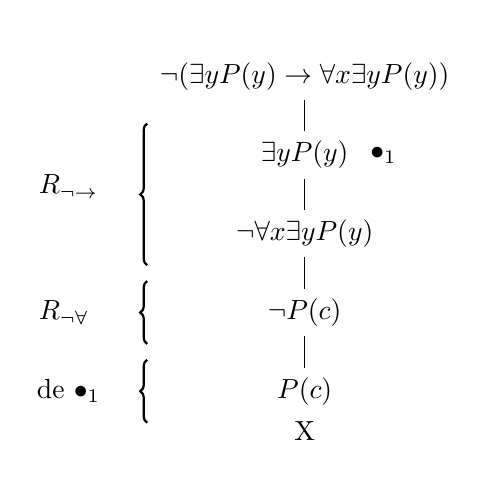
\begin{tikzpicture}
\node at (0,0.5) (dummy) {};%%Para dejar un rengl�n
\node at (0,0) (formula1){$\neg (\exists y P(y) \rightarrow \forall x \exists y P(y))$};
\node at (0,-1) (formula2) {$ \exists y P(y)$}; \node at (1,-1) (1) {$\bullet_1$};
\node at (0,-2) (formula3) {$\neg \forall x \exists y P(y)$};
\node at (0,-3) (formula4) {$\neg P(c)$};
\node at (0,-4) (formula5) {$P(c)$};
\node at (0,-4.5) (fin) {X};

\draw [-] (formula1) to (formula2);
\draw [-] (formula2) to (formula3);
\draw [-] (formula3) to (formula4);
\draw [-] (formula4) to (formula5);

\draw [decorate,decoration=brace,thick]  (-2,-2.4) -- (-2,-0.6);
\draw [decorate,decoration=brace,thick] (-2,-3.4) -- (-2,-2.6);
\draw [decorate,decoration=brace,thick] (-2,-4.4) -- (-2,-3.6);
\node at (-3,-1.4) (nodo1) {$R_{\neg \rightarrow}$};
\node at (-3,-3) (nodo2) {$R_{\neg \forall}\ $};
\node at (-3,-4) (nodo3) {de $\bullet_1$};
\end{tikzpicture}
\end{center}
\end{enumerate}
\end{enumerate}